The user here provides information about the building and the units
the user will work with. The widget contains 4 separate frames,
as shown in \Cref{fig:gi_overview}:

\begin{enumerate}
\item Building Information: Collects general information about the building: name, type, and year of construction.
\item Properties: Collects information about number of stories, width, depth, plan area and height of the building.
\item Location: Collects information about the location of the building. This information is used in some event widgets to obtain events specific to the building location.
\item Units: Collects information about the units for the inputs and outputs. Some widgets will require inputs in different units. Those widgets will display units beside those special entry fields.
\end{enumerate}

\begin{figure}[!htbp]
  \centering {
    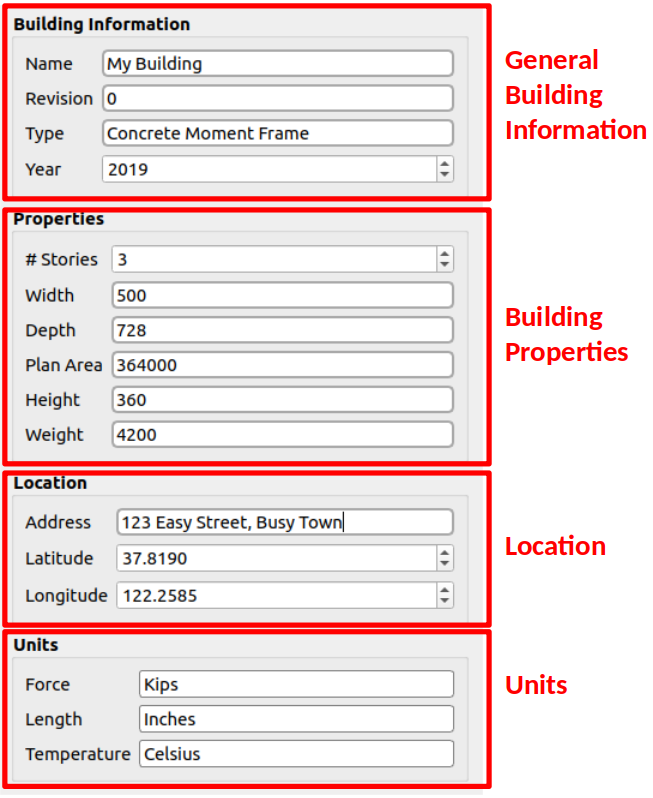
\includegraphics[width=0.5\textwidth]
    {usage/figures/gi.png} }
  \caption{General Information Input Panel}
  \label{fig:gi_overview}
\end{figure}

